\documentclass[doktyp=barbeit, sprache=german]{TUBAFarbeiten}
\usepackage[utf8]{inputenc}
\usepackage[T1]{fontenc}
\usepackage{graphicx} 
\usepackage{amsmath}
\usepackage{subcaption}
\usepackage{algorithm}
\usepackage{algorithmicx}
\usepackage[noend]{algpseudocode}
\newcommand*\rfrac[2]{{}^{#1}\!/_{#2}}
\captionsetup{compatibility=false}
\bibliographystyle{unsrt}
\TUBAFFakultaet{Fakultät für Mathematik und Informatik}
\TUBAFInstitut{Institut für Informatik}
\TUBAFLehrstuhl{Lehrstuhl für Künstliche Intelligenz und Datenbanken}
\TUBAFTitel{Eine Studie zur kombinatorischen Optimierung mit Ameisenalgorithmen}
\TUBAFBetreuer{Prof. Dr. H. Jasper}
\TUBAFKorrektor{M. Sc. V. Göhler}
\TUBAFAutor[S. Dressel]{Samuel Dressel}
\TUBAFStudiengang{Angewandte Informatik}
\TUBAFVertiefung{Künstliche Intelligenz}
\TUBAFMatrikel{59\,963}
\TUBAFDatum[2018-11-05]{05. November 2018}
\begin{document}
\maketitle
\tableofcontents
\newpage
\section{Einleitung}
\section{Grundlagen}
\subsection{Der Ameisenalgorithmus (Ant Colony Optimization)}
\subsubsection{Biologische Grundlagen}
Grundlage der Erörterung über die Funktionsweise des Ameisenalgorithmus bildet sicherlich ein Blick auf die biologischen Grundlagen. Dabei spielt die Kommunikation der Ameisen untereinander die zentrale Rolle. Ein Tierstaat wie er bei den Ameisen zu finden ist funktioniert nur mit einer effektiven und sinnvollen Kommunikation. Methoden zur Verständigung wie das Kommunizieren über Vibrationen und Berührungen sind eher die Ausnahme und kommen nur in speziellen Situationen zum Tragen (\cite{Ameisen}). Dagegen wird zum größten Teil der Informationsaustausch über Duftstoffe (sog. Pheromone) bevorzugt. Diese werden durch verschiedene Drüsen erzeugt und wiederum in unterschiedlicher Kombination und Konzentration abgegeben.
Diese Pheromone werden zum einen benutzt, um Nestgenossen zu erkennen oder um bei Gefahren Kampf- und Abwehrverhalten auszulösen. Hauptsächlich jedoch nutzen Ameisen die Pheromone um eine Duftspur über ihren Hinterleib abzugeben. Diese dienen ihnen und ihren Nestgefährten als Orientierungshilfe. Zum einen werden damit Straßen zu anderen Kolonien gebildet - zum anderen dient es dazu, anderen Ameisen den Weg zu einer Nahrungsquelle zu zeigen. Die Tatsache, dass ein Weg mit einer höheren Pheromonkonzentration bevorzugt wird, ist Grundlagen des Ameisenalgorithmus.
\subsubsection{Der Ameisenalgorithmus}
Der historische Ursprung des Algorithmus findet sich in den Versuchen von Jean-Louis Deneubourg und seine Kollegen (\cite{Biological}). Das sogenannte "Double-Bridge-Experiment" zeigte, dass Ameisen den kürzesten Weg aufgrund der Pheromonmarkierung finden. In dem Experiment ist eine Kolonie von Argentinischen Ameisen durch zwei Brücken mit einer Nahrungsquelle verbunden (\cite{Dorigo2007}). Dabei können die Ameisen die Futterquelle nur über diese zwei Brücken erreichen. Im ersten Teil des Versuchs sind diese beiden Brücken jeweils gleich lang (Abbildung \ref{img:DBExperiment}a). Zu Beginn erkunden die Ameisen die Umgebung der Kolonie bis sie eine Entscheidung über die Auswahl der Brücke treffen müssen. Lässt sich aufgrund einer noch nicht stattgefundenen Begehung der Brücken keine Pheromonspur feststellen, so entscheiden die Ameisen rein zufällig welche Brücke sie wählen. Die Wahrscheinlichkeit für beide Wege liegt bei gleichen Bedingungen bei ca. 50 Prozent. Wird der Versuch über längere Zeit durchgeführt, so wird durch Zufall die Pheromonkonzentration der einen Brücke höher sein als die andere. Diese wird dadurch attraktiver für die Ameisen und wird somit letztenendes der favorisierte Weg zur Nahrungsquelle. Im zweiten durchgeführten Versuch sind die beiden Brücken unterschiedlich lang (Abbildung \ref{img:DBExperiment}b). Auch hier liegt die Wahrscheinlichkeit für beide Brücken zu Anfang bei ca. 50 Prozent. Da die Ameisen, die sich für die kürzere Brücke entscheiden, schneller wieder zuirück am Nest sind, steigt das Pheromonlevel auf diesem Weg deutlich schneller an. Nach einigen Iterationen kristalliert sich die kürzere Brücke als optimale Route heraus, während der längere Weg durch Pheromonreduktion immer unattraktiver wird. Im Vergleich zum ersten Versuch geschieht dieser Prozess wesentlich schneller und effektiver.
\begin{figure}
\captionsetup[subfigure]{justification=centering}
\centering
\begin{subfigure}[c]{0.45\textwidth}

\includegraphics[width=0.9\textwidth]{images/RouteTrivial.png}
\subcaption{Skizze zu Versuch 1; beide Wege sind gleich lang}
\end{subfigure}
\begin{subfigure}[c]{0.45\textwidth}
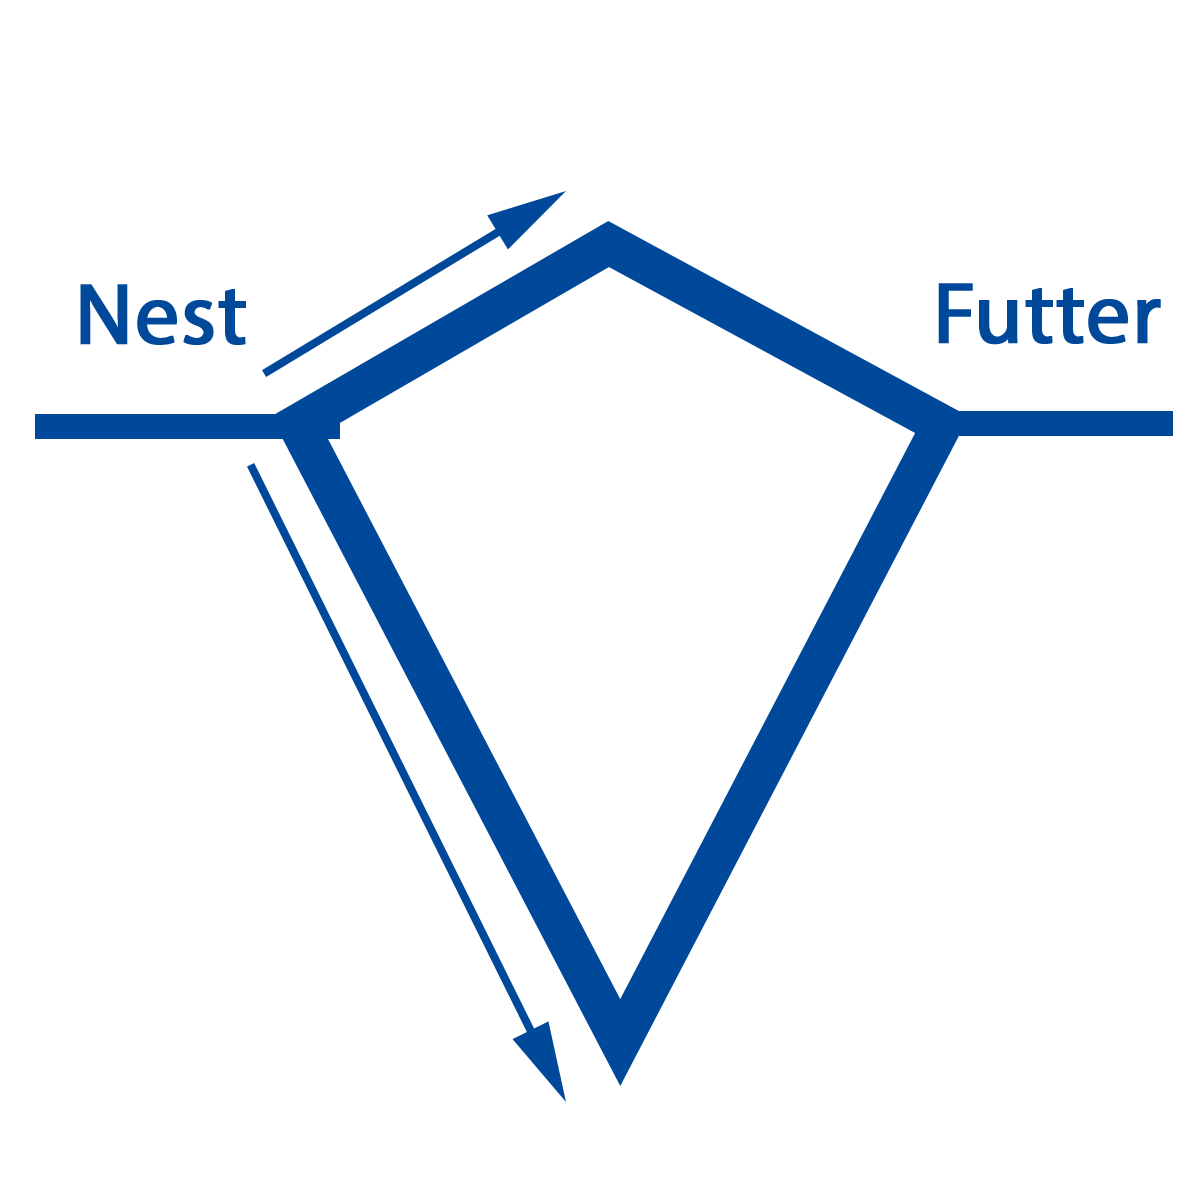
\includegraphics[width=0.9\textwidth]{images/RouteAdv.png}
\subcaption{Skizze zu Versuch 2; die Wege sind unterschiedlich lang}
\end{subfigure}
\caption{Double-Bridge-Experiment}
\label{img:DBExperiment}
\end{figure}
\subsection{Das Travelling-Salesman-Problem}
\subsubsection{Das Problem im Allgemeinen}
Das Travelling Salesman Problem (im Folgenden mit TSP abgekürzt) ist eines der bekanntesten und meist untersuchten Optimierungsprobleme (\cite{TaschenbuchAlgorithmen}). Die Aufgabe, mit der sich das Problem beschäftigt, ist folgende: Ein Handlungsreisender soll in einer Rundreise \(n\) verschiedene Städte besuchen. Der Reisende startet dabei (zufällig) in einer dieser Städte und am Ende seiner Reise kehrt er auch wieder in diese Stadt zurück. Dabei sollen alle Städte nur einmal besucht werden und dabei die Weglängen bzw. die Kosten minimiert werden.\\Formal lässt sich dieses Problem mathematisch so definieren: $G = (V,E)$ sei Graph und $F$ die Menge aller Hamiltonkreise in $G$. Dabei beschreibt $V = \{1,...,n\}$ die Menge der Knoten, $E$ die Menge der Kanten. Für jede Kante $e \in E$ existierten ein Wert $c_e$, der die Gewichtung/die Kosten für diese Kante beschreibt. Diese Kosten als Kostenmatrix $C = (c_{ij})_{n\times n}$ dargestellt werden, dabei entspricht jeder Eintrag $c_{ij}$ den Kosten der Kante, die den Knoten $i$ mit dem Knoten $j$ verbindet. Ziel ist das Finden des Hamiltonkreises $f \in F$, für den die Summe der einzelnen Kantenkosten minimal wird (\cite{TSPVariations}).
\\Seinen geschichtlichen Ursprung hat das TSP im Jahr 1832, als in Deutschland ein Buch mit dem Titel "Der Handlungsreisende, wie er sein soll und was er zu thun hat, um Aufträge zu erhalten und eines glücklichen Erfolges in seinen Geschäften gewiss zu sein" erschien. Dieses Buch und dessen Inhalt definierte die Grundlagen des Problems.  Die erste Benutzung des Ausdrucks "Traveling Salesman Problem" ist nicht ganz geklärt; in mathematischen Kreisen war dies in den Jahren 1931 - 1932 der Fall. (\cite{TSP}). 
Dies geschah als mehrere amerikanische Mathematiker sich des Problems annahmen - wichtige Vertreter waren dabei Merrill FLood und Hassler Whitney, die dort die Überlegungen des österreichischen Mathematikers Karl Menger als Grundlage nahmen. Nach und nach wurde das Problem durch zahlreiche Veröffentlichungen immer präsenter und bis heute ist das TSP eines der schwierigsten und prominentesten Probleme in der Mathematik.
\\Unter der bislang unbewiesenen Annahme, dass die Komplexitätsklassen $P$ und $NP$ verschieden sind,gehört das TSP zur Klasse der NP-vollständigen Probleme, was bedeutet dass es sich nicht mit einem deterministischen Algorithmus in Polynomialzeit lösen lässt (\cite{Applegate2007}).  Alle ansatzweise effektiven Möglichkeiten und Algorithmen zur Lösung des TSP sind deshalb nichtdeterministisch. 
\subsubsection{Ansätze und Algorithmen zur Lösung des Problems}
Da das Problem wie oben schon erwähnt zu den NP-vollständigen Problemen gehört, gibt es keinen effizienten Algorithmus der bei einer hohen Anzahl von Städten eine optimale Tour findet. (\cite[p.~150]{TSP}). Entweder ist ein Algorithmus zur Lösung des TSP schnell oder er findet eine optimale Tour - aber er wird nicht beide Eigenschaften besitzen. Deswegen unterscheidet man wie auch allgemein bei anderen kombinatorischen Optimierungsproblemen zwischen exakten und heuristischen Algorithmen.
Der einfachste Algorithmus zur exakten Lösung des TSP ist die sogenannte \textit{"brute-force\grqq} \, oder naive Methode (\cite{TaschenbuchAlgorithmen}). Dieser Algorithmus betrachtet nacheinander alle möglich Touren und deren Länge und ermittelt durch den Vergleich derselben die optimale und kürzeste Tour. 
Ist der Graph \(G\), der dieses Problem modelliert, ein ungerichteter Graph, so muss man mit diesem Algorithmus \(\frac{1}{2} \cdot (n - 1)!\) verschiedene Rundreisen betrachten. Bei neun verschiedenen Städten ergeben sich daraus 20160 verschiedene Touren, bei 16 Städten dagegen schon 653 Milliarden Routen, was diesen Algorithmus für die meisten Optimierungsprobleme völlig unbrauchbar macht. Auch andere exakte Methoden haben dennoch oft einen hohen Rechen- und Zeitaufwand. Man entscheidet sich deswegen häufig dafür effiziente heuristische Algorithmen zu konstruieren, die zwar keine optimale Tour finden, aber zumindest eine annäherungsweise optimale Tour. Es existieren eine Vielzahl von solchen heuristischen Verfahren - eines der intuitivsten ist dabei der \textit{Nearest-Neighbor-Algorithmus} (\cite{Lotz2014}). Hierbei wird ein zufälliger Knoten $v_1$ als Startknoten asugewählt. Danach wird iterativ immer der Knoten $v_i$ ausgewählt, der dem zuletzt ausgewählten Knoten am nächsten liegt und noch nicht in der schon besuchten Knotenmenge $V^\prime$ enthalten ist. Der Algorithmus ist beendet, wenn alle Knoten besucht wurden. Das Problem hierbei ist, dass die letzte Kante, die den letzten Knoten mit dem Startknoten verbindet und den Hamiltonkreis vervollständigt, eine mehr oder weniger beliebige Länge haben kann und somit die Optimalität der gefundenen Lösung wesentlich einschränkt. Formal lässt sich der Algorithmus wie folgt darstellen: 
\begin{algorithm}
\caption{Nearest-Neighbor-Algorithm}
\label{euclid}
\textbf{Eingabe:} $G = (V,E,c)$
\\\textbf{Ausgabe:} Tour $V_C$, die alle Knoten $v \in V$ besucht
\begin{algorithmic}[1]
\State $z_1 := v \in V$
\State $V^\prime := V \, \backslash \, \{v_1\}$
\State $i := 2$
\While {$V^\prime \ne \emptyset$}
\State $z_1 := min_{v\in V^\prime}  \, c(\{v_{i-1},v\})$
\State $V^\prime := V^\prime \, \backslash \, \{v_i\}$
\State $i := i +1 $
\EndWhile
\State $V_C := (v_1,...,v_n,v_1)$
\end{algorithmic}
\end{algorithm}
Ein weiterer bekannter heuristischer Algorithmus ist die \textit{Minimal-Spaaning-Tree-Heuristik, kurz MST}. Dabei wird zunächst ein minimaler Spannbaum $B$ für den Graphen $G$ ermittelt (\cite{Groetschel2005}). Zur Ermittlung dieses minimalen Spannbaumes stehen mehrere Algorithmen zur Verfügung (Algorithmus von Prim, Algorithmus von Kruskal, ...) (\cite{MST}). Danach wird jede Kante innerhalb des Spannbaumes verdoppelt; es entsteht eulersche Graph $G^\prime$. Nun wählt man einen beliebigen Startknoten und folgt den Kanten im Sinne einer Eulertour. Bereits besuchte Kanten werden dabei gestrichen und stattdessen die direkte Verbindung zwischen den jeweils verbleibenden Knoten gewählt. Das \textit{Verfahren von Christofides} baut auf diesem Algorithmus und erweitert diesen dadurch, dass der minimale Spannbaum nicht verdoppelt wird, sondern das minimale Matching von den Knoten in $B$ sucht, die einen ungeraden Grad haben. Nach der Dreiecksungleich gilt, dass die Summe der Längen zweier Seiten $a$ und $b$ stets mindestens so groß ist wie die Länge der dritten Seite (formal: $c \leq a + b$). Die MST-Heuristik ist deswegen höchstens doppelt so lang, die Christofides-Heuristik höchstens höchstens 1,5-mal so lang wie die optimale Lösung(\cite{Groetschel2005}).
\subsubsection{TSPLIB als Quelle für bekannte Probleme} \label{TSPLIB}
Die in dieser Arbeit untersuchten Probleme stammen aus der TSPLIB der Universität Heidelberg. Bekannte Probleme wurden dort in ein einheitliches Datenformat gebracht und eignen sich deswegen gut zur Auswertung von Implementierungen des TSP. Vor allem die Existenz der Daten als XML-Datei (Extensible Markup-Language-File) vereinfacht die Anwendung der Lösungsalgorithmik auf viele verschiedene Probleme sehr einfach (\cite{TSPLIB}).
\subsubsection{Möglichkeiten der Distanzberechnung}
Um das TSP lösen zu können benötigt man Informationen über die Distanzen bzw. die Wegkosten zwischen den einzelnen Knoten. In der TSPLIB (\ref{TSPLIB}) sind dabei die Kantenwerte schon berechnet worden. Dieser Berechnung hängt vom Format der Positionsinformationen der einzelnen Knoten ab. Die zwei wichtigsten Distanzarten, die auch den Daten in dieser Arbeit zu grade liegen, sind die \textit{Euklidische Distanz} und die \textit{Geographische Distanz}. Die Euklidische Distanz (auch euklidischer Abstand) ist der triviale Abstand zwischen zwei Punkten den man auch durch Messung mit einem einfachem Längenmessgerät wie einem Lineal ermittelt (\cite{Distanz}). Die Distanz $d_{xy}$ der Punkte $x$ und $y$ in einer Ebene mit den Koordinaten $x = (x_1, x_2)$ und $y = (y_1, y_2)$ ergibt sich dabei aus folgender Formel:
\begin{align}
\label{eq:Euclid}
d_{xy} = \left\| x - y \right\|_2 = \sqrt{{(y_1-x_1)}^2+{(y_2-x_2)}^2}
\end{align}
Die Ermittlung der geographischen Distanz ist dagegen etwas komplizierter. Dies hat die Ursache, dass die Koordinaten im Fall der Erde auf einer Kugel liegen. Betrachtet man die Erde als ideale Kugel mit einem Radius $r = 6378,388 \,km$ und liegen die Koordinaten in der Dezimalschreibweise vor, ergibt sich für die für zwei Städte $i$ und $j$ folgende Berechnung:
\begin{algorithm}
\caption{Geographische Distanz}
\label{geodistance}
\begin{algorithmic}[1]
\State $r = 6378,388$
\State $latitude_i = latitude_i \cdot \pi / 180; \,latitude_j = latitude_j \cdot \pi / 180$
\State $longitude_i = longitude_i \cdot \pi / 180;\, longitude_j =longitude_j \cdot \pi / 180$
\State $q_1 = cos(longitude_i - longitude_j)$
\State $q_2 = cos(latitude_i - latitude_j)$
\State $q_3 = cos(latitude_i + latitude_j)$
\State \textbf{$d_{ij} = r * arccos(0,5 \cdot ((1 + q_1) \cdot q_2 - (1 - q_1) \cdot q_3)) + 1)$}
\end{algorithmic}
\end{algorithm}
\subsection{Das Travelling-Salesman-Problem und der Ameisenalgorithmus}
Betrachtet man den Ameisenalgorithmus bzw. das Ant Colony Optimization Problem - so ähnelt dies dem TSP sehr stark. Dies war auch der Grund, warum der Ameisenalgorithmus zuerst als Lösung für das TSP zur Anwendung kam.
\\Es bietet sich an, dass TSP hierzu als Graphenproblem zu modellieren (\cite{MaxMin}):
Hat mein ein TSP mit $n$ Städten, so benötig man neben einer $n\times n$-Matrix $D$ mit den verschiedenen Distanzen zwischen den Knoten auch einer $n\times n$-Matrix $T$ mit den verschiedenen Pheromonkonzentrationen. Dabei ist das Element $\tau_{ij}$ die Pheromonkonzentration auf der Kante zwischen Knoten $i$ und $j$, analog ist die Distanz $d_{ij}$ die Distanz zwischen den Knoten $i$ und $j$. Ist das verwendete TSP symmetrisch, dann ist auch die Pheromonspur symmetrisch; das heißt: $\tau_{ij} = \tau_{ji}$.
Abstrakt gesehen werden dann zunächst alle $m$ Ameisen einer Menge $M$ auf verschiedene zufällig gewählte Knoten gesetzt. Danach bewegt sich jede Ameise $m_k$ in jedem darauffolgenden Iterationsschritt zu einem weiteren Knoten, falls sie diesen vorher noch nicht besucht hat und insgesamt nicht alle Knoten schon besucht wurden. Der Entscheidung, welcher Knoten als nächstes besucht wird, liegen gewisse Regeln zugrunde. Zum einen hat die Pheromonkonzentration der jeweiligen Kanten zu den anderen Knoten Einfluss auf die Entscheidung, zum anderen die heuristische Information $\eta_{ij}$. Die heuristische Information ergibt sich dabei aus der Distanz:
\begin{align}
\label{eq:Heuristic}
\eta_{ij} = \rfrac{1}{d_{ij}}
\end{align}
Bei der Wahl des nächsten Knotens bevorzugen die Ameisen solche Knoten, die relativ nah gelegen sind und die durch eine Kante mit hoher Pheromonkonzentration verbunden sind.
Die Wahrscheinlichkeit, mit der eine Ameise $k \in M$ ausgehend von eines Knotens $i$ den nächsten Knoten $j$ besucht, kann durch folgende Gleichung ausgedrückt werden:
\begin{align}
\label{eq:Prob}
p^k_{ij} = \frac{[\tau_{ij}]^\alpha \, [\eta_{ij}]^\beta}{\sum\nolimits_{l\in N^k_i} [\tau_{il}]^\alpha \, [\eta_{il}]^\beta} \; \; \text{if}\: j \in N^k_i
\end{align}
Dabei sind $\alpha$ und $\beta$ Parameter, die im Fall von $\alpha$ die Wichtigkeit der Pheromonkonzentration und im Fall von $\beta$ die Wichtigkeit der Distanzinformationen zur Entscheidungsfindung angeben. $N^k_i$ ist die Menge der erreichbaren Knoten der Ameise $m_k$, wobei diese Menge die Menge der unbesuchten Knoten darstellt. Jede Ameise merkt sich zudem die Reihenfolge der besuchten Knoten in einer Liste. Falls eine Ameise $m_k$ alle Knoten $n$ besucht hat, kehrt sie zu ihrem Anfangsknoten zurück und beendet ihre Tour. Anhand der Liste mit den besuchten Knoten lässt sich nun ein valider Hamiltonkreis ableiten. Außerdem ist diese Liste notwendig, um die Pheromonkonzentration der benutzten Kanten zu aktualisieren.
\\Für ein Pheromonupdate gibt es verschiedene Möglichkeiten, die für 2. bis 4. im Rahmen dieser Bachelorarbeit auch umgesetzt wurden: 
\begin{enumerate}
\item Aktualisierung des Pheromonlevels nachdem alle Ameisen ihre Tour beendet haben
\item Aktualisierung des Pheromonlevels iterativ nach der erfolgreichen Tourkonstruktion jeder einzelnen Ameise $m_k$
\item Aktualisierung des Pheromonlevels für alle Ameisen $m \in M$ parallel, nachdem der jeweils nächste Knoten erreicht wurde
\item Aktualisierung des Pheromonlevels nur durch die Ameise, welche nach Beendigung der Tour den kürzesten Weg gefunden hat
\end{enumerate}
Die Berechnung der neuen Pheromonkonzentration auf einer Kante $\tau_{ij}$ zum Zeitpunkt $t + 1$ ist für alle Varianten gleich und berechnet sich wie folgt:
\begin{align}
\label{eq:Pheromone}
\tau_{ij}(t+1) = \rho \, \tau_{ij}(t) + \sum_{k=1}^m \Delta \tau^k_{ij}(t)
\end{align}
$\Delta \tau^k_{ij}(t)$ stellt dabei die Menge an Pheromon dar, die eine Ameise $k$ auf der jeweilige Kante $\{i,j\}$ ablegt. $1-\rho$ ist die verfliegende Menge an Pheromon. Dieser Verdunstungsmechanismus, der durch den Parameter $\rho$ gegeben ist, hilft dabei, ungünstige Kanten mit der Zeit zu \glqq vergessen\grqq. 
\section{Implementierung des Problems in C++}
\subsection{Programmstruktur und Funktionsweise}
\subsection{Vorgehensweise zur Untersuchung von verschiedenen Datensätzen mit verschiedenen Implementierungen}
\section{Ergebnisse der Durchführung}
\subsection{Resultate bei Iteration einzelner Ameisen nacheinander}
\subsection{Resultate bei paralleler Erschließung}
\section{Auswertung und Vergleich}
\subsection{Vergleich der iterativen und parallelen Implementierung}
\subsection{Vergleich mit der optimalen Lösung}
\subsection{Vergleich mit der Laufzeit und Komplexität von anderen Algorithmen}
\section{Zusammenfassung und Fazit}
\section{Anhang}
\newpage
\bibliography{literatur}{}
\addcontentsline{toc}{section}{Literatur} 
\end{document}